\section{Estimates of arrival time}
\label{sec:eta_estimates}

As previously discussed, there is considerable uncertainty in the posterior predictive distribution of arrival time. This uncertainty makes point estimates challenging to provide since there is a strong negative correlation between \emph{accuracy}---how far the estimates are from the actual value---and \emph{reliability}---how \emph{useful} the estimate is. Take for example the median, which has, on average, the highest accuracy, but 50\% of the time the bus arrives earlier than the estimate, which could lead to a passenger missing their bus. To overcome this, we also explore using \emph{prediction intervals} to balance accuracy and reliability.

The method for obtaining estimates from the \glspl{cdf} from \cref{sec:etas_cdfs} uses quantiles, such that the $q$-quantile, $q\in(0,1)$, is found by
\begin{equation}
\label{eq:eta_calc_quantile}
\max\{a : \Pr{A < a} \geq q\}
\end{equation}
\Cref{fig:eta_calc_quantile} shows a single \gls{cdf} with a horizontal line at $q$, and the largest ETA with its quantile below this line is the desired value; in this case, $\hat A_{0.5} = 11$.


\begin{knitrout}
\definecolor{shadecolor}{rgb}{0.969, 0.969, 0.969}\color{fgcolor}\begin{figure}

{\centering 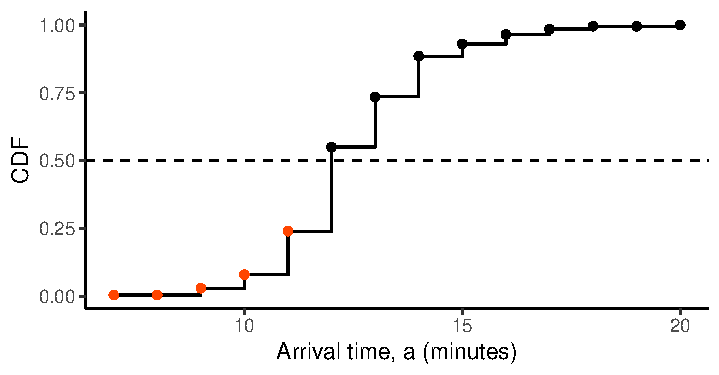
\includegraphics[width=.8\textwidth]{figure/eta_calc_quantile-1} 

}

\caption[Quantile estimation from a CDF]{Quantile estimation from a CDF. ETA values with quantiles below the desired threshold are coloured red; the maximum of these is the quantile value.}\label{fig:eta_calc_quantile}
\end{figure}


\end{knitrout}


\subsection{Point estimate}
\label{sec:etas-point}

In a perfect world, it would be possible to predict precisely how long it would take a bus to arrive at a stop, and display this single number to passengers. Alas, as we saw in \cref{cha:prediction}, this is not a perfect world, and arrival time prediction inherently comes with significant uncertainty. Yet we still need to decide on the best single value to use as a point estimate of arrival time, since much of the infrastructure currently available only allows this. We also want to examine if it is possible to come up with a single statistic that performs well---on average---and, more importantly, better than the currently deployed method.





\begin{knitrout}\small
\definecolor{shadecolor}{rgb}{0.969, 0.969, 0.969}\color{fgcolor}\begin{figure}

{\centering 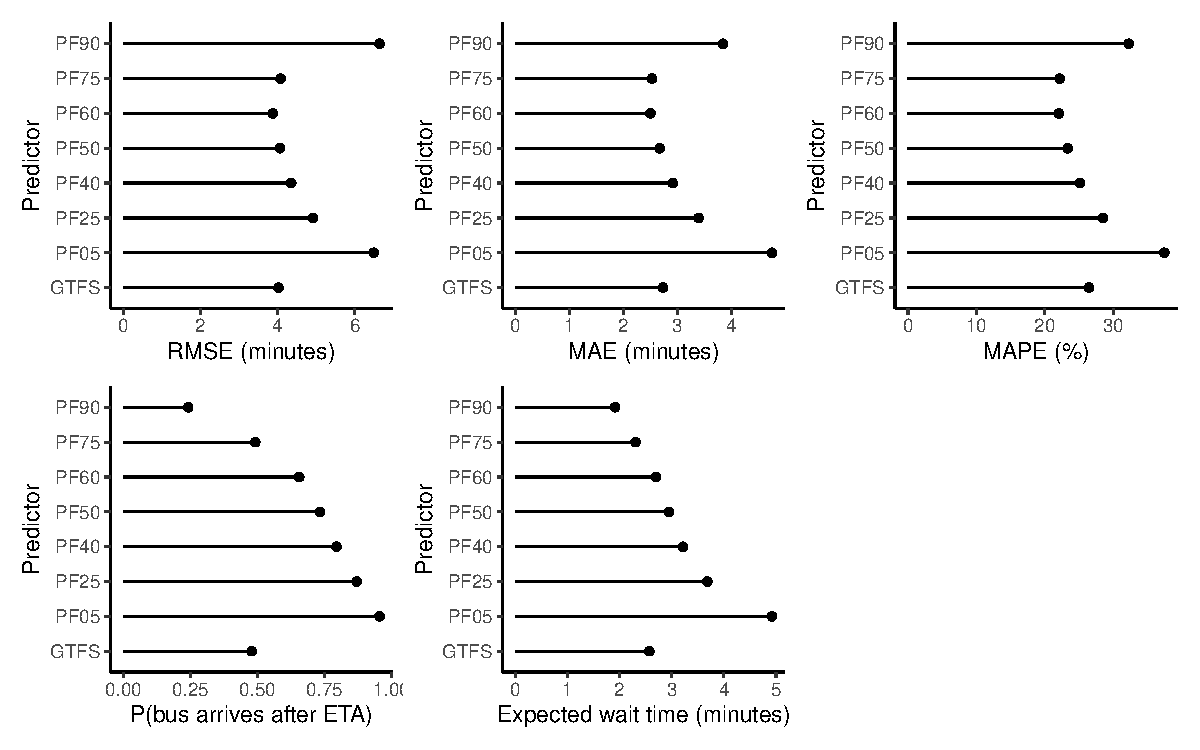
\includegraphics[width=\textwidth]{figure/eta_overall_results-1} 

}

\caption[Comparison of summary statistics for various quantiles of the predictive distribution, and the currently deployed GTFS method]{Comparison of summary statistics for various quantiles of the predictive distribution, and the currently deployed GTFS method. Results are displayed for all day average, and off-peak (between 9h30 and 14h30).}\label{fig:eta_overall_results}
\end{figure}


\end{knitrout}


We calculated, for all stops, trips, and times, a range of arrival times quantiles ($q \in \{0.05, 0.25, 0.5, 0.6, 0.6, 0.75, 0.9\}$), and for each computed the \gls{rmse}, the probability of catching the bus given you arrive at the stated \gls{eta}, $\Pcatch$, and the expected waiting time given you catch the bus, $\Ewait$. The results are displayed in \cref{fig:eta_overall_results}, along with the same values computed used the \gls{gtfs} arrival time estimates. For the particle filter, the lowest \gls{rmse} value is achieved when using the 60\% quantile, which obtains a 67\% probability of the bus arriving after the \gls{eta} and an expected waiting time of 2.7~minutes. The coverage of the quantiles are being overestimated---we would expect the 60\% quantile to have an approximately 40\% success rate---which indicates that the current implementation of the particle filter is underestimating arrival times.


\begin{knitrout}\small
\definecolor{shadecolor}{rgb}{0.969, 0.969, 0.969}\color{fgcolor}\begin{kframe}


{\ttfamily\noindent\bfseries\color{errorcolor}{\#\# Error in eval(lhs, parent, parent): object 'c05' not found}}\end{kframe}
\end{knitrout}

An important consideration is the cost of missing the bus. For each trip, we computed the scheduled time between the current trip and the subsequent one (which is termed \emph{headway}) to compute the expected waiting time if the bus arrives \emph{before} the predicted time. That is, if a bus is predicted to arrive in 5~minutes, but actually arrives in 3, and the time until the next bus (servicing the same trip) is 10~minutes, then the expected waiting time will be $10-5=5$~minutes (assuming the passenger arrives in 5~minutes). This \emph{headway} is an essential component to prediction cost.

The total expected wait time can be conditioned on whether or not the bus was caught,
\begin{equation}
\label{eq:eta_wait_conditional}
\begin{split}
\E{\text{wait}} &=
  \Pr{\text{catch}} \E{\text{wait}|\text{catch}} +
  (1 - \Pr{\text{catch}}) \E{\text{wait}|\text{miss}} \\
  &= \Pr{A \geq a} \E{A - a | A \geq a} +
  \Pr{A < a}\E{\text{headway} - a + A | A < a}
\end{split}
\end{equation}
where $a$ is the estimated arrival time, and $A$ is the actual. For simplicity, we assume headway is maintained (which it is not, \citet{})---that is, if a bus has 20~minute frequency and you miss the bus by 5~minutes, your expected waiting time is 15~minutes.

\Cref{fig:eta_headway_results} shows the values of $\Pcatch$, $\Ecatch$, $\Emiss$, and $\Ewait$ by headway (rounded down, in minutes). Capture probability is not so affected by headway, though it decreases slightly for longer headways. In contrast, expected wait times are very much affected. Most unexpectedly, $\Ecatch$ decreases with headway, which could be caused by a higher proportion of short headway at peak times when traffic is more congested, leading to more uncertainty (so the quantiles are more dispersed), or the buses take longer than expected. For $\Emiss$, the expected wait time is not unexpectedly strongly correlated with headway. Overall, the difference in $\Ewait$ between predictors is negligible for headways less than 10~minutes, after which time differences appear. Low frequency routes should prefer a low quantile to reduce the chance of missing the bus.


We did not examine time-until-arrival, which we saw in the previous chapter explained a lot of the variation in predictor performance. We would expect a similar result here, so if one wanted to develop a predictor based on both headway and time until arrival, that would be straightforward enough. However, it is clear that the choice of predictor is tightly linked with the cost of a bad prediction: is waiting at the bus stop too long more costly than missing it altogether?

\subsection{Interval estimate}
\label{sec:etas-interval}


Deciding on a ``best'' single-value estimate of arrival time is exceedingly difficult given the amount of uncertainty involved. The best approach above is to use a small quantile, but this increases expected wait time given catching the bus (top-right of \cref{fig:eta_headway_results}). An alternative approach is to provide \emph{two} estimates---a lower and upper bound---that is to say, a \emph{prediction interval}. Such an interval should be both \emph{reliable} and \emph{useful} for commuters.

Reliability means that, if one arrives by the \emph{lower estimate}, there is only a small probability of missing the bus. The bus should also have a low chance of arriving after the \emph{upper estimate}, for example when using the prediction to decide which bus to catch to get to a destination on time (more of this in \cref{sec:etas-journey-planning}).

Usefulness corresponds to the width and expected wait time: these should both be minimised where possible, so for example, if a bus is 5~minutes away, providing a 30~minute interval should only be done if there is a good reason to do so. If there is a layover between the bus and the stop, for example, the time range could very well be that large since the particles implement the layover behaviour discussed in \cref{sec:prediction_arrival_time}.







In this section, we consider symmetric prediction intervals of the form $(\Teta_{\alpha/2}, \Teta_{1-\alpha/2})$ where $\alpha \in (0,1)$ gives a $100(1-\alpha)$\% interval. Note that although these intervals are symmetric in probability, they are most often asymmetric on the arrival time scale, particularly when the bus is near, and the distribution is right-skewed, as shown in \cref{fig:eta_dist_skew}. In contrast, a Kalman filter implementation assumes Gaussian errors, so a symmetric interval is also symmetric around the mean, as shown in \cref{fig:eta_dist_skew}, often leading to incorrect intervals (potentially even an \gls{eta} below zero).


\begin{knitrout}\small
\definecolor{shadecolor}{rgb}{0.969, 0.969, 0.969}\color{fgcolor}\begin{figure}

{\centering 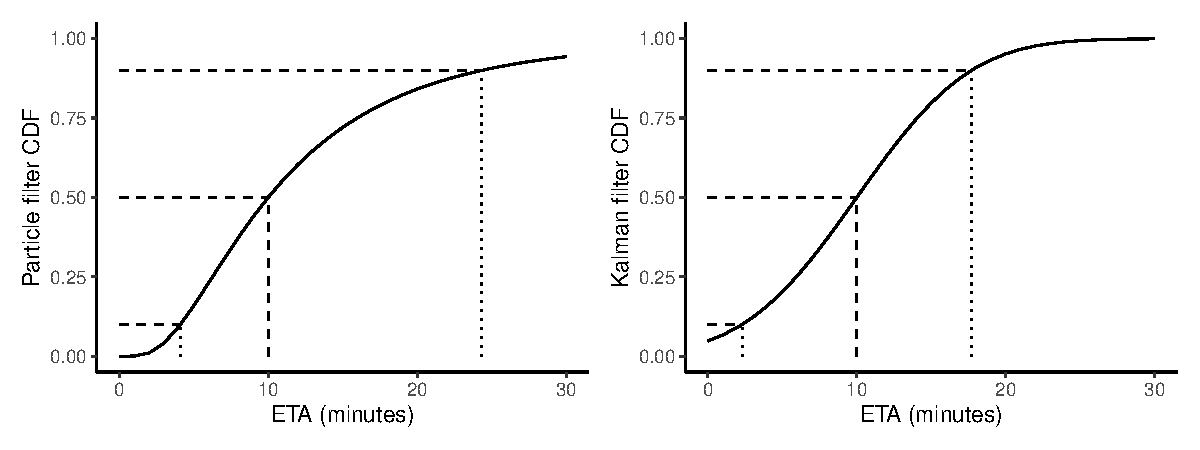
\includegraphics[width=\textwidth]{figure/eta_dist_skew-1} 

}

\caption[Symmetry of arrival time intervals]{Symmetry of arrival time intervals. Symmetric intervals on the probabilty scale map to asymmetric under the particle filter (left), and symmetric intervals under the Kalman filter (right).}\label{fig:eta_dist_skew}
\end{figure}


\end{knitrout}


\begin{knitrout}\small
\definecolor{shadecolor}{rgb}{0.969, 0.969, 0.969}\color{fgcolor}\begin{figure}

{\centering 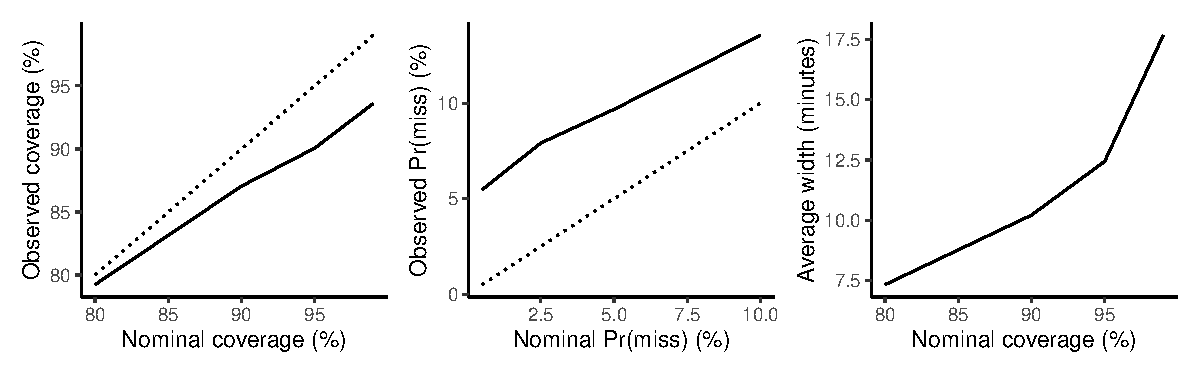
\includegraphics[width=\textwidth]{figure/eta_cis-1} 

}

\caption[ETA CIs]{ETA CIs}\label{fig:eta_cis}
\end{figure}


\end{knitrout}



We computed intervals for $\alpha \in \{0.01, 0.05, 0.1, 0.2\}$, and for each evaluated the observed coverage, the proportion of times that the bus arrived before the lower bound, and the average interval width (in minutes). \Cref{fig:eta_cis} shows that the observed coverage drops slightly as the interval width increases (smaller $\alpha$) and that the probability of the bus arriving before the lower bound is higher than expected, which could indicate that not enough uncertainty is being incorporated. Interval width increases rapidly with coverage probability, demonstrating the trade-off between reliability and usefulness.


Other variables---time until arrival, time of day, or stop sequence---are not considered as we did in the previous chapter, as the results are much the same. However, if desired, such relationships could be explored to choose the best point or interval estimate under any given situation. The goal of this section was to demonstrate that reliability and usefulness can be improved upon by using prediction intervals.

\begin{itemize}
\item I think I might need more discussion here ...
\end{itemize}

